\subsubsection{Future research agenda}
\begin{wrapfigure}{r}{140pt}
    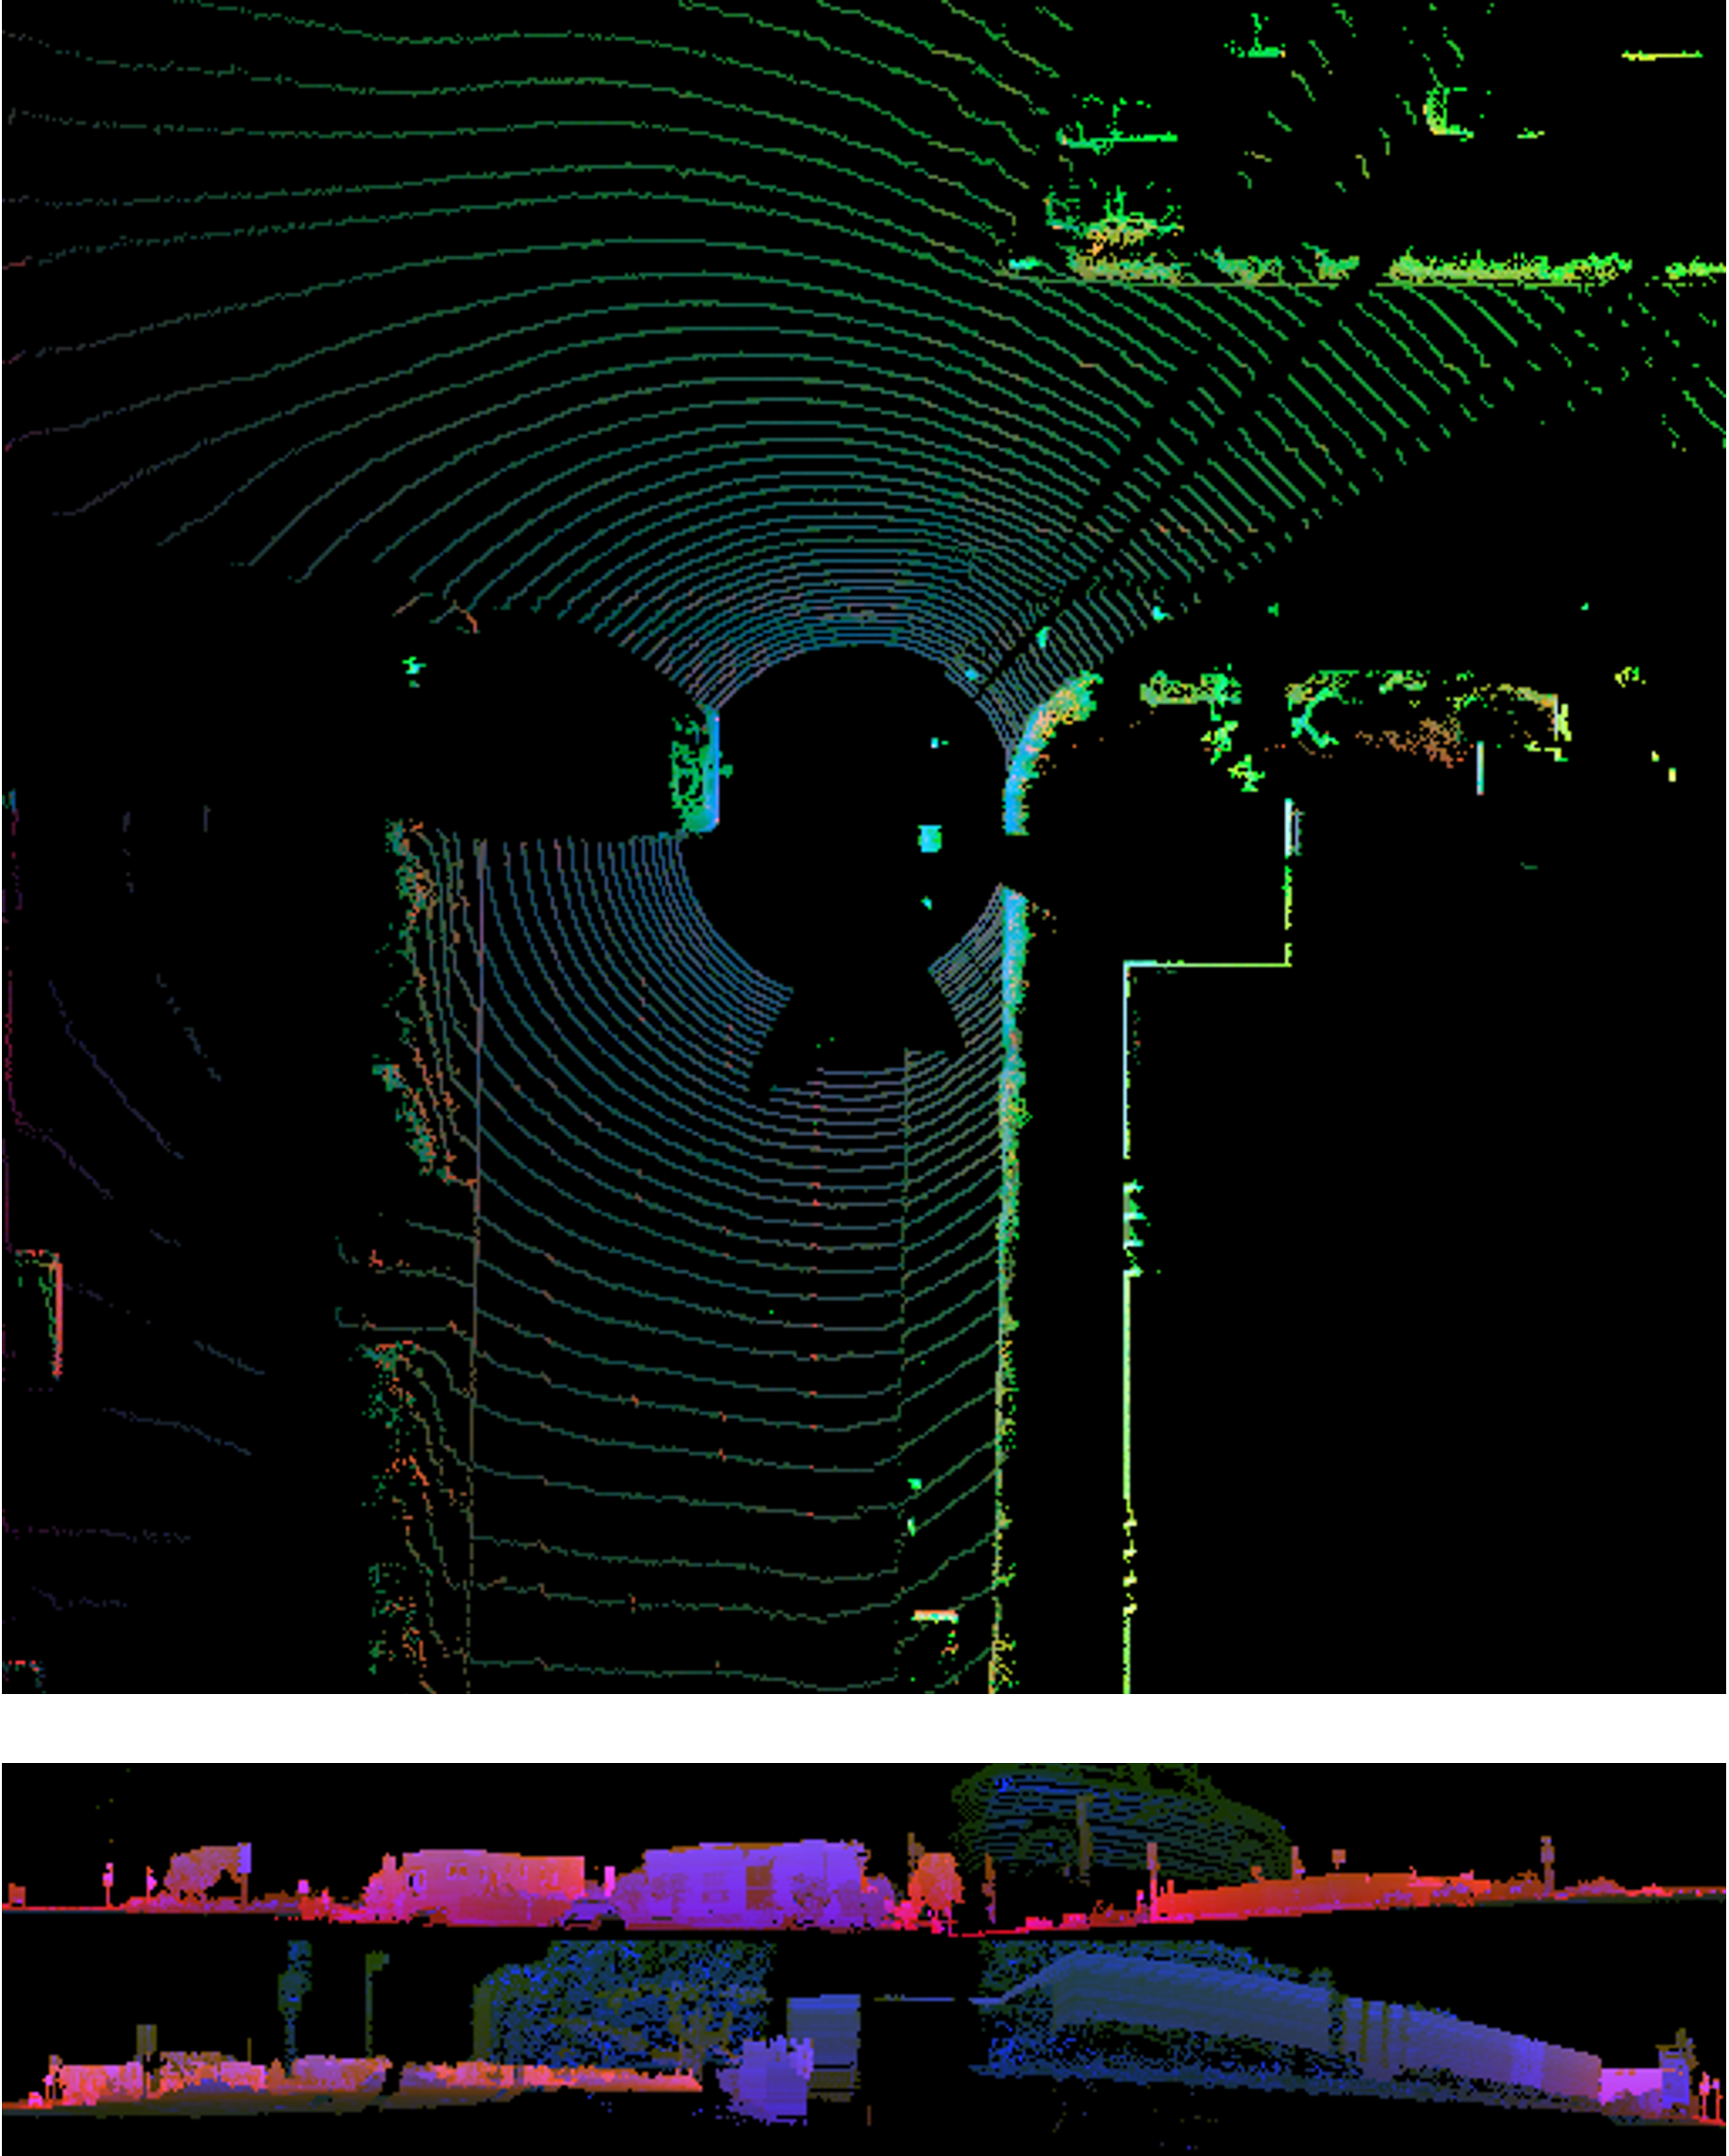
\includegraphics[width=140pt]{pic/fusion.png}
    \mainfont\fontsize{9pt}{9pt}\selectfont\caption{ \mainfont\fontsize{9pt}{9pt}\selectfont Multi View Fusion with Bird's Eye (top)
    and Spherical View (bottom)}
    \label{fig:fusion}
    \end{wrapfigure}
In the future I plan to continue my research in the field of machine learning and computer vision 
especially perception, object detection and the general machine learning methods.
Today representation learning by masking is a technique applied not just in natural language or image modeling 
but also in domains like point cloud representation, trajectory prediction and others. In my future research 
I am keen to not only explore the possibilities of
masked modeling, but also other
self-supervised and semi supervised learning techniques. 
I believe that innovative training strategies such as
regularizing via multi task and curriculum learning will further lead to novel research. 
For example the authors of DAFormer \cite{hoyer} show that
seemingly simple techniques such as rare class sampling, warmup scheduling and additional distillation supervision improve the performance of 
their domain adaptation model.
While the authors of ProFusion3D \cite{valada} showcase an impressive multimodal fusion pipeline, they 
also focus on training strategies via additional objectives in the pretraining phase. 
Noise prediction, cross-modal depth prediction and cross-modal intensity prediction are used on top of the MAE reconstruction objective.

Since the development of pixelNeRF \cite{pixelnerf}, I am following the line of research of NeRF and 3D Gaussian representations.
While pixelNeRF solved the problem of conditioning NeRFs on images in real-time, 
3D Gaussian splatting on the other hand allows for fast rendering. With the recent development of methods like MVSplat \cite{mvsplat}
3D Gaussian representations are obtained with only one forward pass. The 3D Gaussians are a unique 
latent space for 3D scene representations.
The authors of S4C \cite{s4c} use a NeRF to perform 3D semantic scene completion 
without the need for 3D annotations in a smart self-supervised manner. Similarly I would like to explore the use of 
3D Gaussian representations to perform real-time 2D semantic segmentation
3D semantic scene completion within one model. While the 2D semantic segmentation can be rendered from the 3D Gaussian representation,
the 3D semantic scene completion can be derived directly from the 3D Gaussian representation.
